\documentclass[twocolumn]{preport}
\usepackage[dvipdfmx]{graphicx}
\graphicspath{{figs/}}

\renewcommand{\figref}[1]{Fig.\ref{#1}}

\title{ヒューマノイドにおける環境認識に基づく自律歩行計画と行動実現に関する研究}
\author{大森悠貴,指導教員:稲葉雅幸教授 岡田慧教授 \\
キーワード: humanoid, footstep planning, force sense, uneven ground, }

\begin{document}

\pagestyle{empty}
\maketitle
\thispagestyle{empty}
\sloppy

\section{本研究の背景と目的}
% 本稿はプログレスレポートのテンプレートである\cite{Sakai}.
% 本稿における「、」や「。」は、\verb|make pub|を実行することで、「,」や「.」に変更される。
% 図は\figref{nowprinting}や\tabref{sample}として参照する.
近年,災害現場など不整地を含む場所で,脚を持つ特性を活かしてヒューマノイドが人間に代わり,作業を遂行することが期待されている.タスクを行うためには不整地環境において適切に歩行計画を行い,タスクを行う場所まで移動することが不可欠である.

環境認識に基づくヒューマノイドの歩行計画は盛んに研究されてきた\cite{ueda2014biped}が,LiDARなどによる足場環境の形状情報のみを用いるものが多く,足場の形状情報を足探り行動により知る研究などもある\cite{wiedebach2016walking}が,物体の材質による変形可能性などを考慮していなかった.本研究では,足場物体形状に加え,材質情報も用いることにより,適切な歩行計画を行うと同時に,足探り行動により足場環境を確認することで転倒することなく目的地まで到達できるシステムを提案する.

\section{視覚情報と触覚情報を統合した安全度による自律移動システム}
本研究では,足場環境を足場物体の形状・材質・配置の3つの観点から分類し,形状・材質情報は物体の種類に紐付けられるという仮定のもと,物体認識により物体をラベル付けし,そのラベルを用いて足場とした際の安全度を取得する.安全度を歩行計画に用いることで,より安全な足場を選んで目的地まで到達することが出来る.安全度は安全度データベースに記憶されており,物体ラベルと各物体の安全度の情報を持つが,これは安全度が未知の物体が歩行計画された経路に存在する場合,足探り行動によって確かめられる.これにより,安全度が未知の物体については足探り行動により安全度を推定でき,既知の物体は安全度データベースから安全度を取得することで,効率的かつ安全に歩行計画と目的地到達が実現できる.本研究の全体システムを\figref{system}に,初期位置から目的地到達までの一連の流れを\figref{flowchart}に示す.

\begin{figure}[tbh]
  \begin{center}
    \begin{minipage}{0.63\columnwidth}
      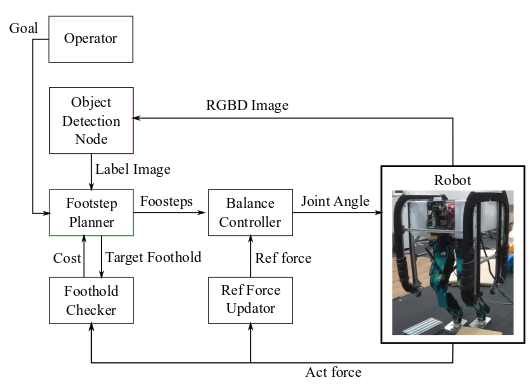
\includegraphics[width=0.95\columnwidth]{system.png}
      \caption{全体システム図}
      \label{system}
    \end{minipage}
    % \hspace{0.15\columnwidth}
    \begin{minipage}{0.35\columnwidth}
      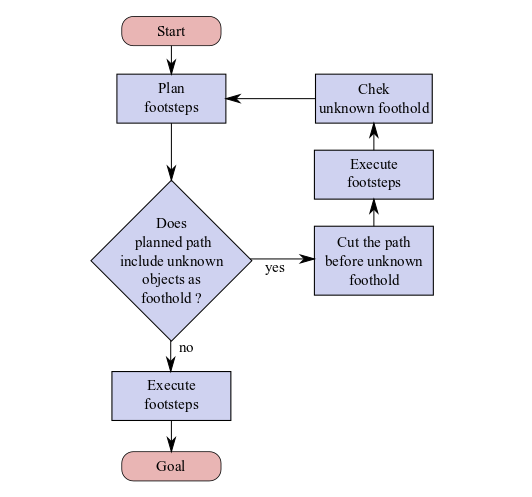
\includegraphics[width=0.95\columnwidth]{flowchart.png}
      \caption{初期位置から目的地到達までの流れ}
      \label{flowchart}
    \end{minipage}
  \end{center}
\end{figure}


\section{足場環境の安全度を用いた歩行計画}
歩行計画は,A支持脚に対する遊脚の配置可能領域を離散化することでグラフ探索問題として考えられ,A*アルゴリズムを用いることにより実現されている.三次元環境での歩行計画は,二次元環境での座標を環境の三次元点群に射影し,着地可能判定を行うことにより実現されている.A*アルゴリズムでは,ヒューリスティック関数と実コスト関数により次に探索するノードが決定される.本研究では,歩数コストに加え,安全コストをこれらのコスト関数に組み込むことにより,安全コストの高い,つまり足場としては安全ではない物体を避けて目的地までの経路計画を行うようにした.

\section{足探り行動による足場環境の安全度推定}
未知の物体が歩行経路に存在した場合,転倒することなく目的まで到達するためには,その物体が足場として適切かどうかを調べる必要がある.本研究では,物体を踏むことでその物体の材質情報を取得することを足探り行動と呼び,これにより安全度を推定した.本研究では,足探り行動の動作を作成し,足探り行動を行う遊脚の目標反力を更新することにより,転倒することなく確認物体の反力を足裏力センサにより取得した.

\section{安全度を用いた歩行計画と目的地到達の実現}
足場としての安全度の低いスポンジと,安全度の高い金属フレームのどちらかを歩行経路に含む必要のある環境を用意し,全ての物体を未知/既知とした時に歩行計画をし,目的地まで到達する実験を行った.
未知物体が歩行経路に含まれた場合に,未知物体の手前を中継目的地に設定し,目的地到達後に足探り行動を行う様子を\figref{checksoft}に示す.ここでは,全ての物体が未知の条件で歩行計画を行ったため,面積の大きいスポンジが足場に選ばれている.足探り行動により,安全度データベースが更新されている.また,安全度データベース更新後に同じ目的地に対して歩行計画を行い,目的地まで到達する様子を\figref{stephard}に示す.ここでは安全度の高い金属フレームが足場に選ばれている.

\begin{figure}[tbh]
  \centering
  \begin{minipage}{0.24\columnwidth}
    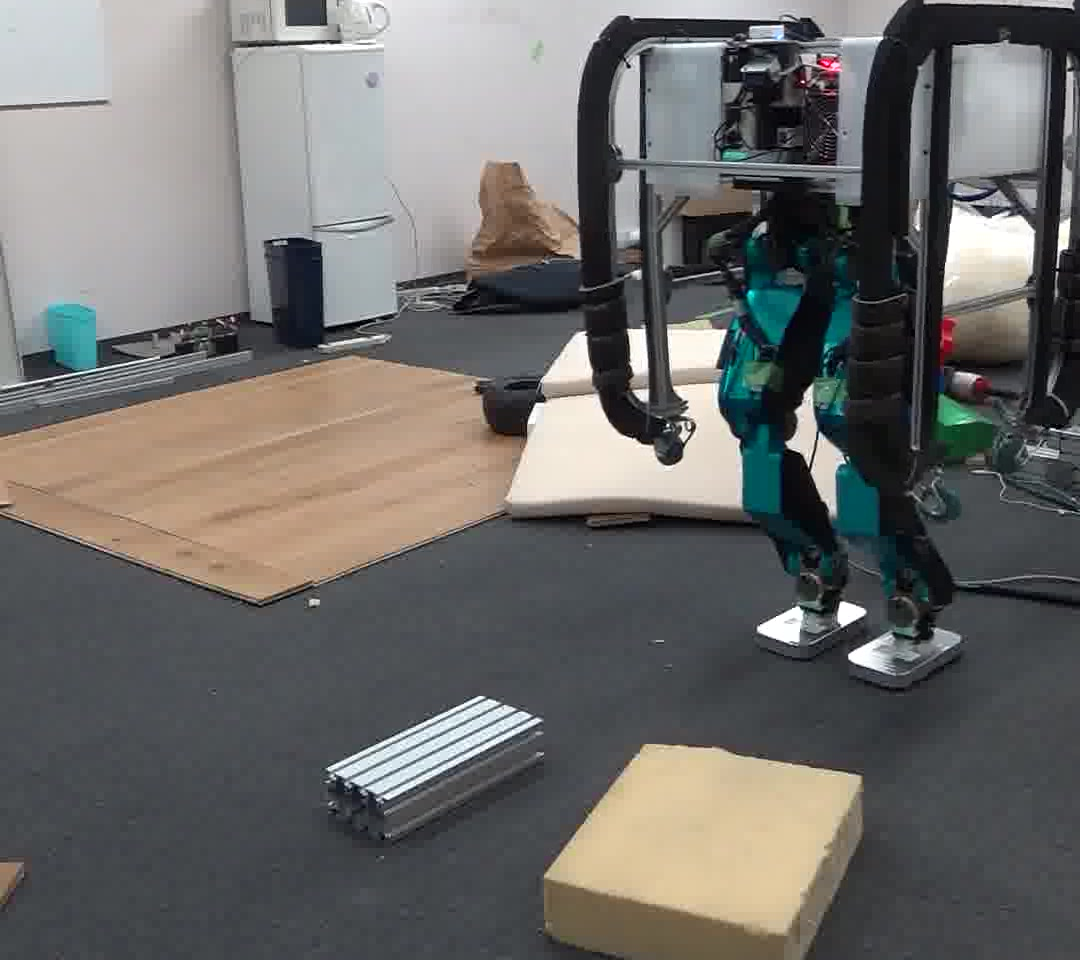
\includegraphics[width=0.95\columnwidth]{checksoft05}
  \end{minipage}
  \begin{minipage}{0.24\columnwidth}
    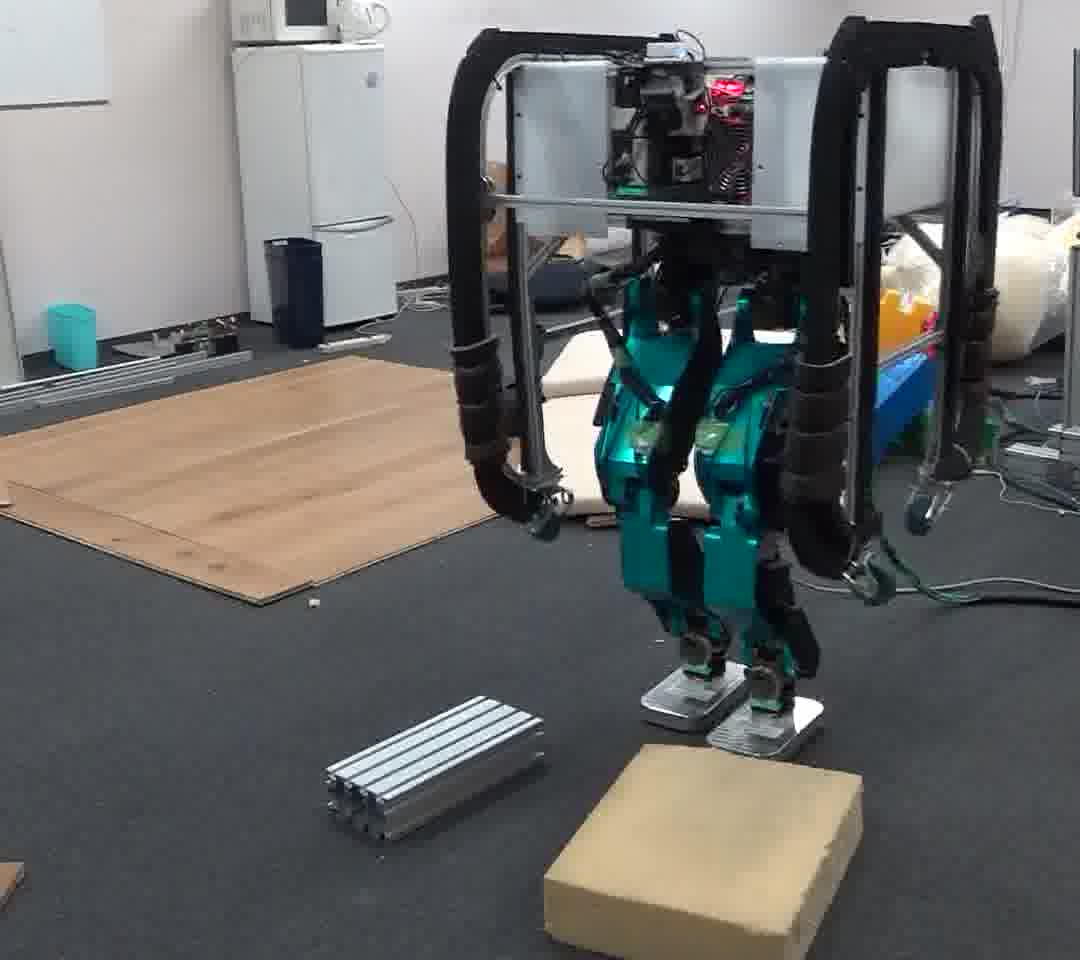
\includegraphics[width=0.95\columnwidth]{checksoft13}
  \end{minipage}
  \begin{minipage}{0.24\columnwidth}
    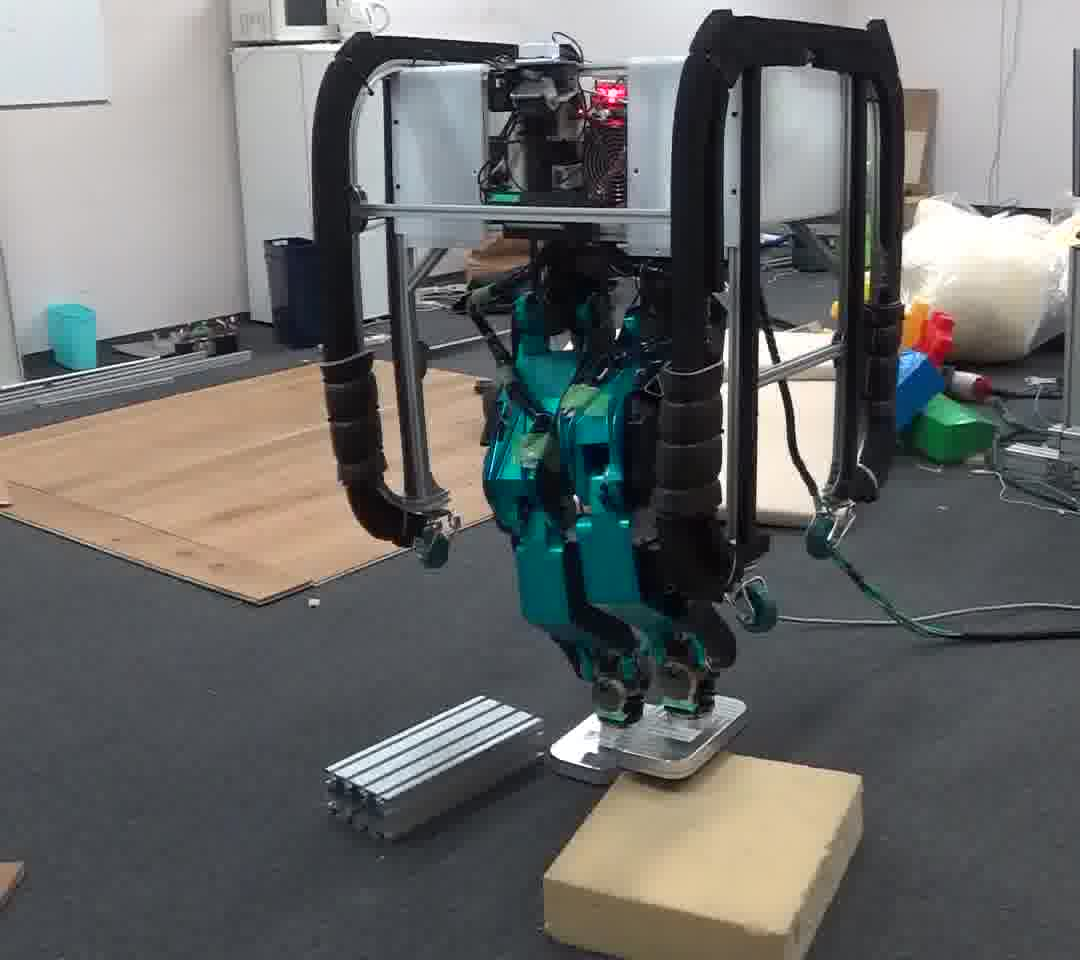
\includegraphics[width=0.95\columnwidth]{checksoft63}
  \end{minipage}
  \begin{minipage}{0.24\columnwidth}
    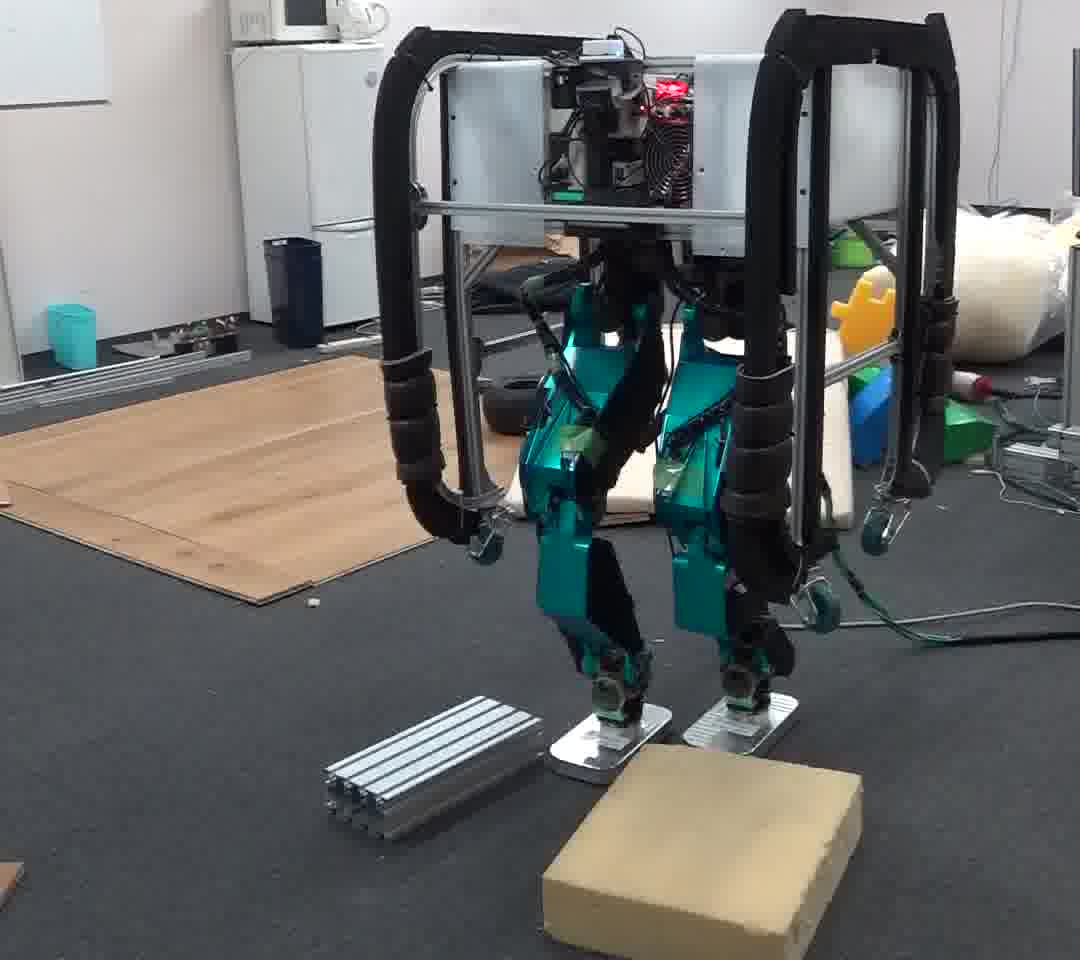
\includegraphics[width=0.95\columnwidth]{checksoft123}
  \end{minipage}
  \caption{未知物体手前まで行き足探り行動を行う様子}
  \label{checksoft}
\end{figure}

\begin{figure}[tbh]
  \begin{center}
    \begin{minipage}{0.24\columnwidth}
      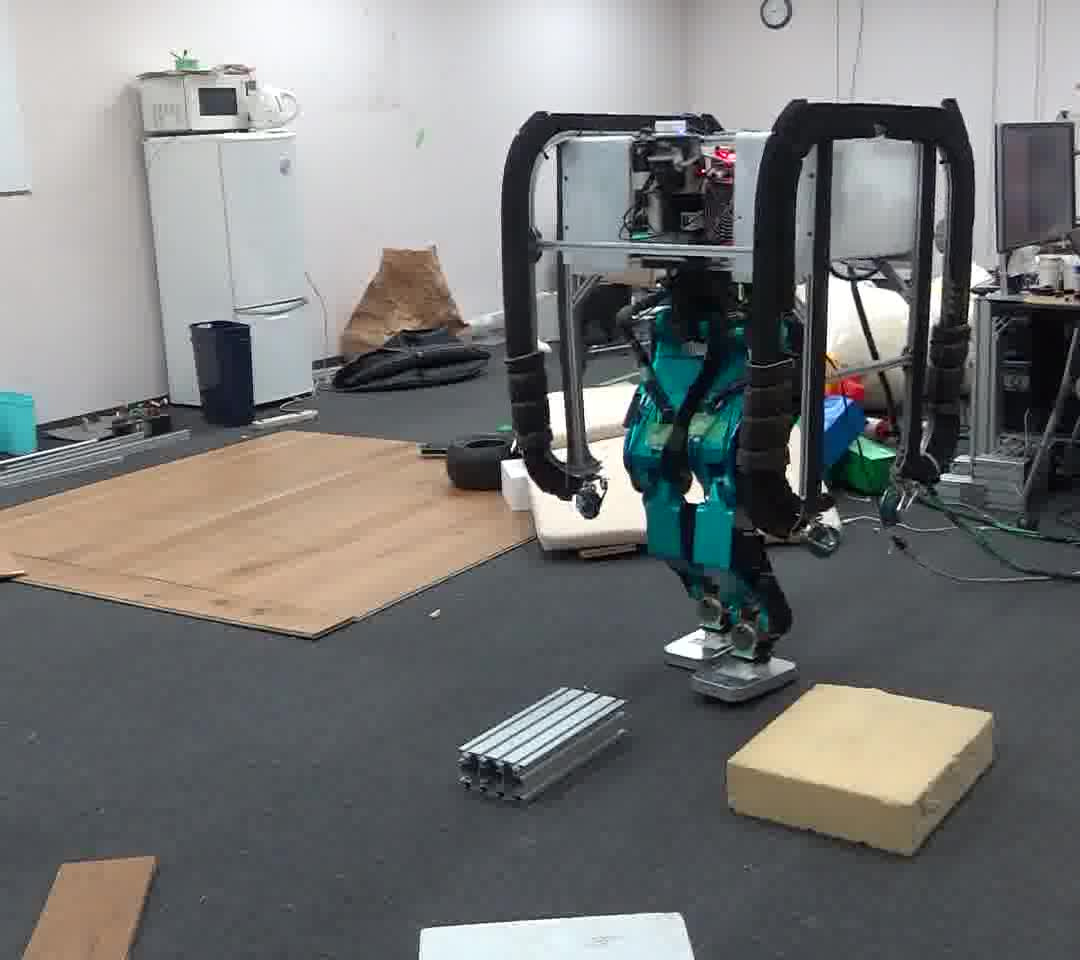
\includegraphics[width=0.95\columnwidth]{stephard09}
    \end{minipage}
    \begin{minipage}{0.24\columnwidth}
      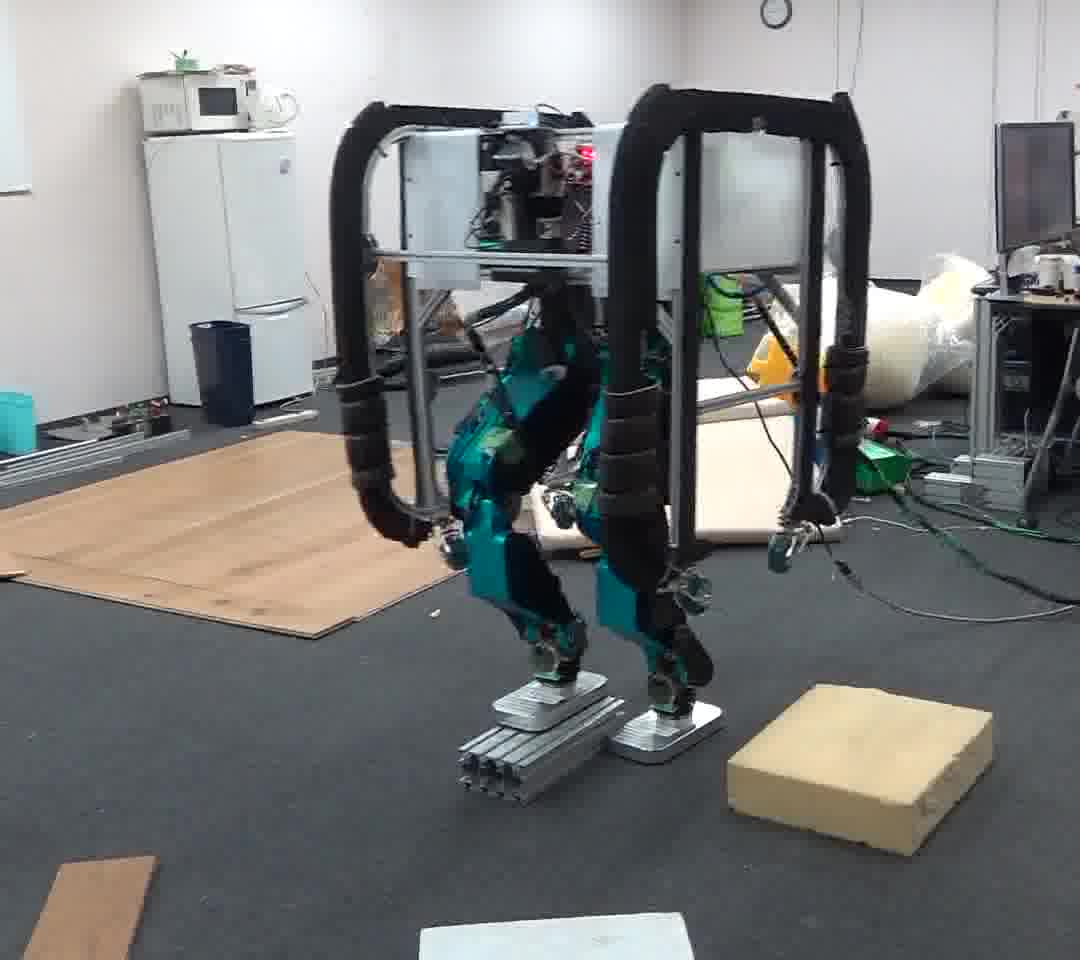
\includegraphics[width=0.95\columnwidth]{stephard13}
    \end{minipage}
    \begin{minipage}{0.24\columnwidth}
      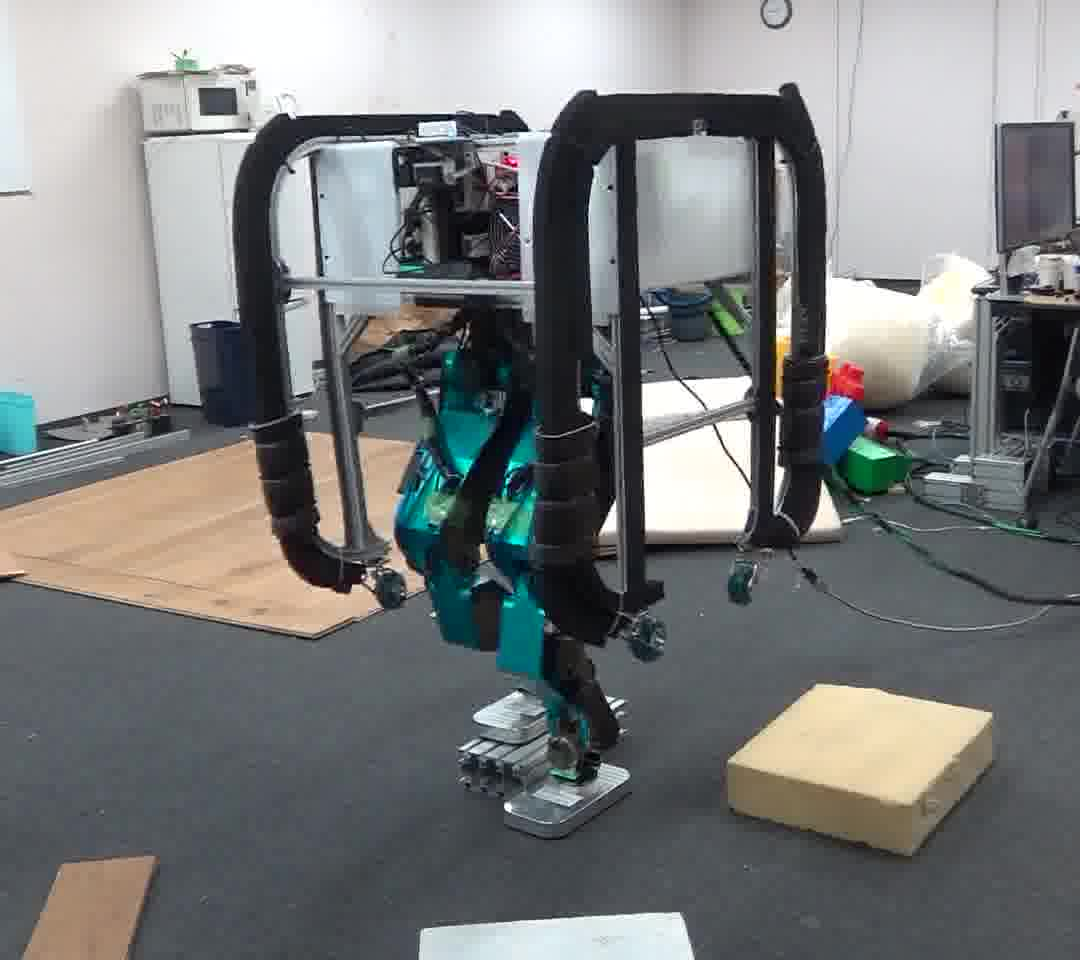
\includegraphics[width=0.95\columnwidth]{stephard17}
    \end{minipage}
    \begin{minipage}{0.24\columnwidth}
      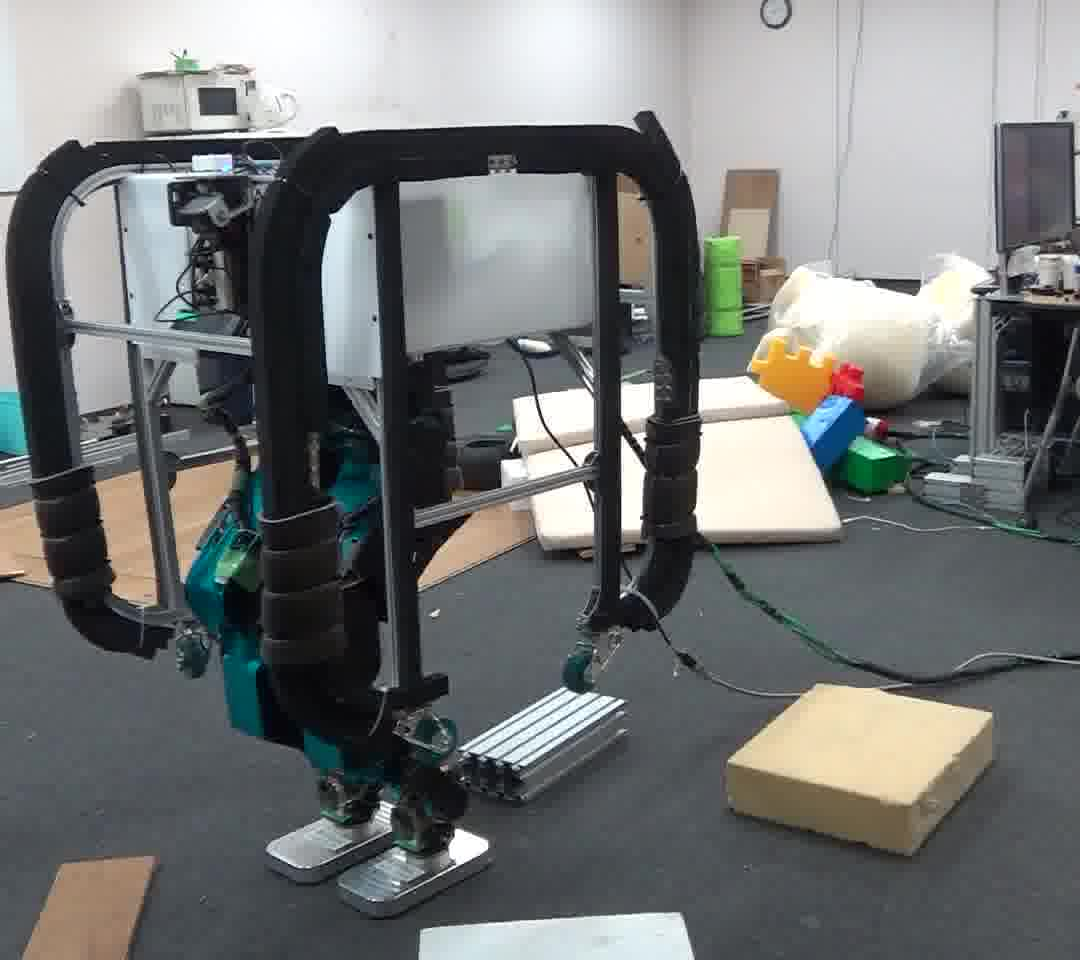
\includegraphics[width=0.95\columnwidth]{stephard25}
    \end{minipage}
    \caption{安全度の高い物体を歩行計画に含め目的地まで到達する様子}
    \label{stephard}
  \end{center}
\end{figure}

% \begin{table}[tbh]
%  \begin{center}
%   \begin{tabular}{|l|r|} \hline
%   A1 & B1 \\
%   A2 & B2 \\ \hline
%   \end{tabular}
%   \caption{図の参考例}
%   \label{table:sample}
%  \end{center}
% \end{table}

\section{本研究の成果と結論}

\bibliographystyle{junsrt}
\bibliography{p-report}

\end{document}
